\documentclass[conference]{IEEEtran}

\usepackage{graphicx}
 \usepackage{amsmath}

\usepackage{xspace} 
\usepackage{hyperref}
% cleverref has to be loaded after hyperref
\usepackage[noabbrev]{cleveref}
\usepackage{color}
\usepackage{amssymb,amsmath}
\usepackage{multirow}


\renewcommand{\quotation}[1]{``\emph{#1}''}

\newcommand{\ie}{\emph{i.e.},\xspace}
\newcommand{\eg}{\emph{e.g.},\xspace}
\newcommand{\etc}{\emph{etc.}\xspace}
\newcommand{\etal}{\emph{et al.}\xspace}

%\usepackage[none]{hyphenat}

\usepackage{paralist}

\newcommand{\nb}[3]{
  \fcolorbox{black}{#2}{\bfseries\sffamily\scriptsize#1}
    {\sf\small$\blacktriangleright$\textit{#3}$\blacktriangleleft$}
}

\newcommand\AB[1]{\nb{alberto}{cyan}{#1}}

\newcommand\odf{\emph{One-day flies}\xspace}

\hyphenation{op-tical net-works semi-conduc-tor}


\begin{document}
\title{One-day flies on StackOverflow\\
{\LARGE Why the vast majority of StackOverflow users only posts once}}



\author{
\IEEEauthorblockN{
Rogier Slag,\IEEEauthorrefmark{1}
Mike de Waard,\IEEEauthorrefmark{2}
Alberto Bacchelli\IEEEauthorrefmark{3}}
\IEEEauthorblockA{
 \{\IEEEauthorrefmark{1}r.g.j.slag,
   \IEEEauthorrefmark{2}m.dewaard\}@student.tudelft.nl,
 \IEEEauthorrefmark{3}a.bacchelli@tudelft.nl}
\IEEEauthorblockA{Delft University of Technology, The Netherlands}}





\maketitle


\begin{abstract}


StackOverflow (SO) is a popular question and answers (Q\&A) platform related to
software development. An interesting characteristic of SO is that about 
half of its users makes only one contribution to the platform in total.

In this work, we study this group of users, which we call \odf, and we 
investigate why they do not continue to contribute to the platform, despite its
growing popularity. By achieving this understanding we can find ways to enable
users to become more active, thus improving the platform. 
\end{abstract}

\IEEEpeerreviewmaketitle



\section{Introduction}

StackOverflow is a Q\&A community on the Internet, which is managed by the
StackExchange platform. It focuses primarily on programming related questions,
and is the biggest Q\&A community on that specific topic.

StackOverflow has been gaining popularity during the last few years
\cite{anderson2012discovering}, and lots of research has been done on the data
corpus of StackOverflow, such as \cite{treude2011programmers},
\cite{barua2014developers} and \cite{morrison2013age}. These and many other
research papers on StackOverflow are about the users personalities
\cite{bosu2013building}, their field of expertise and on how these users
contribute \cite{movshovitz2013analysis}, but not so much research has gone
into how the underlying structure of the StackOverflow community. With
underlying structure we mean, for example the distribution of posts among
users, the distribution of reputation among users, and so on.

This is why we started with some exploratory data analysis on the StackOverflow
Data, which revealed that over $75\%$ of the users posted only twice or even
less during their whole registration period. Given this high amount of
\textit{one-day flies} we analyzed what happens to the content that these
people contribute to the system. The initial idea was that most of these
single-posts could be either marked as duplicate, very specific to a certain
domain / programming language and do not get answered, or reveal a flaw in the
documentation of an API. To elaborate a bit further on the flaw in API
Documentation, a one-day fly can ask a question regarding how to use a specific
API but not have any further questions for StackOverflow as he/she is an
experienced developer. However during this research interesting findings
regarding these initial beliefs emerged.


\section{Related work}

Several aspects of SO have already been investigated, such as how to
build reputation \cite{bosu2013building} and how the reputation system
encourages users to participate \cite{movshovitz2013analysis}. These studies 
gave us insight in how the reputation system works and how this affects the user
base. 
Correa \& Sureka \cite{correa2014chaff} investigated the deletion of
questions on SO; we use this as the basis for verifying some of our hypotheses.
Bazelli \etal analyzed personality traits of SO
users~\cite{bazelli2013personality}; on their work we base our sentimental
analysis for post and answers. 
Yang \etal investigated the group of experts on
SO~\cite{yang2014sparrows}; our work complements theirs by considering a
different group of users.


\section{Defining one-day flies}

As shown by several studies~\cite{yang2014sparrows}, Q\&A platforms are
composed by users with different activity behaviors, which closely follow a
power law distribution: A small set of very highly active users contributes
to the vast majority of the produced content; a larger set of less active users
contributes to fewer parts of the content; and a set (the largest) of users
contributes very little to nothing.

We start our investigation by quantifying the result of this community dynamics
in SO and use it to cluster users and define \odf. We consider the SO data dump
provided for the MSR Challenge 2015~\cite{MSRChallenge2015} and we analyze both
user activity (based on number of posts) and user reputation (based on the
score obtained in the gamification mechanism in place on
SO~\cite{anderson2013steering}).  We find that 47\% of the users made a maximum
of one post, while the most prolific user had 30.043 posts. Similarly, 60\%
(2.063.174) of the users had a reputation of one, the third quartile is 13, and
the maximum value is 709.269.  This is in line with general trends on Q\&A
platforms.

We then apply clustering to users based on their reputation, using k-means;
\Cref{kmeans_clustering} shows how these clusters are averagely placed in terms
of posts and reputation. The largest group of users (3.469.897) is placed in
the bottom-left of the plot; the medium active user group is significantly
smaller (3.012 users) with an average reputation of 38.000;  the group with the
most reputation is by far the smallest (186 users) with a very high average
reputation of ca. 200.000.

With this information, we define \odf as users who posted a maximum of one
question in SO, thus covering both low activity and low reputation. This set
comprises 1.622.688 users, \ie 47\% of the user base. 

\begin{figure}[h]
 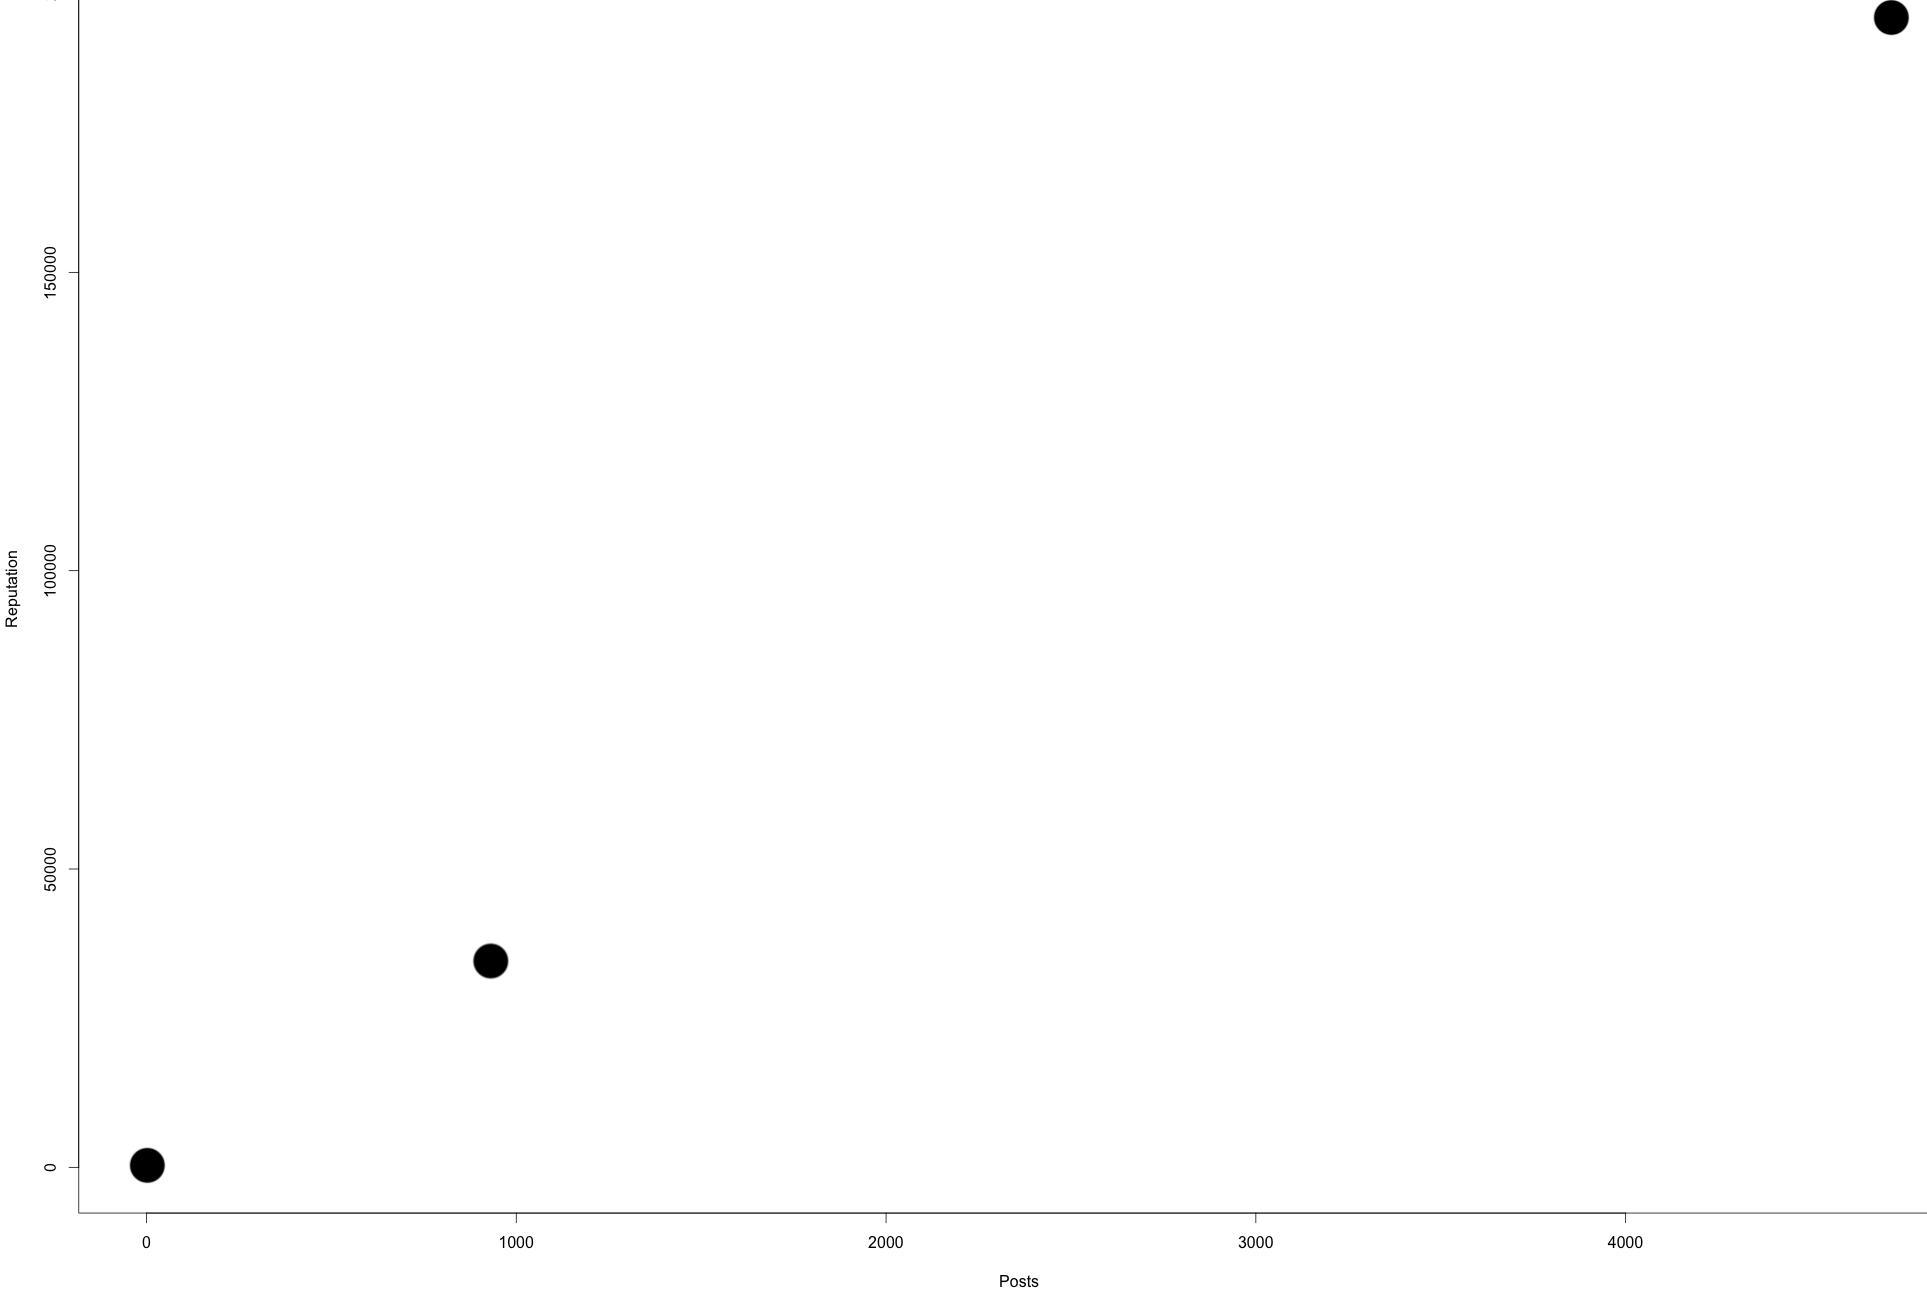
\includegraphics[width=\columnwidth]{clustering.png}
 \caption{The clustering of the user groups}
 \label{kmeans_clustering}
\end{figure}


\section{Experiment}

We conduct an experiment to quantitatively test different hypotheses, expressed
as research questions on what may characterize \odf with respect to other users
of SO. In the experiment we use the complete SO MSR Challenge
dump~\cite{MSRChallenge2015}, imported into a MSSQL database through a
multithreaded data loader we implemented.  For the actual querying, statistical
analysis, and plotting of the data we use a mixture of Ruby (especially to mine
additional data), C\# (to query the data), and R (to perform statistical
analysis and generate plots).  In the following we describe each hypothesis,
with the intuition behind it, the research method we used to test it, and the
results.

\subsection{Duplicate questions}

\textbf{Intuition.} New users who register on
the website could, because of their unfamiliarity with the system, ask
questions that have been asked previously. These questions would be flagged
by the community as \textit{duplicate}. Although this may be the appropriate
action for the community as a whole, it could be extremely discouraging for the
user which posted the question, thus inducing to not post anymore. 

\textbf{RQ1:} Are \odf more likely to create questions marked as duplicates?

\textbf{Research method.} To answer this research question, we compare the
percentage of duplicate questions  between all users and \odf. To do so, we
extract questions asked by \odf and count those marked as duplicate by checking
on  LinkTypeId in the PostLinks table; then we do the same for all questions in
the SO data dump. This holds because the total amount of questions asked by
one-day flies is less than $8\%$ of the complete question set. After retrieving
these results a simple comparison should show whether one day flies post more
duplicate questions in comparison to the complete user base.

\textbf{Results.} The total amount of questions asked by \odf is about 8\%. The
number of duplicate questions is surprisingly low for both groups. One could
expect that this would be high on a public Q\&A community where a large
percentage of the users is unfamiliar with platform. However, only $2.2\%$ of
the one-day flies questions is marked as a duplicate. Meanwhile, this
percentage increases to $2.9\%$ for the regular users. We found this
surprising, since we expected regular users to be more familiar with the
platform and its search functionality. Based on these results, \odf are not
more likely to create duplicate questions than regular users, but slightly
less.


\subsection{Uncommon tags}

\textbf{Intuition.} The topic of a question in SO is commonly translated into
tags, which make it easier for experts to find questions they could answer.
Users who post questions regarding a topic with hardly any experts on the SO
platform can get discouraged by the lack of comments or answers to guide them
into the right direction. This types of topics would be reflected by uncommon
tags accompanying the questions. 
 
\textbf{RQ2:} Are \odf more likely to post questions with uncommon tags?
 
\textbf{Research method.} Correa and Sureka found over $3.300$ tags that only
occur in questions of quality far below StackOverflow
standards~\cite{correa2014chaff}. The answer to our research question is
inspired by their findings, as similar results might be found. We analyze the
top $50$ most popular tags given by \odf questions in comparison to the top
$50$ tags given in all questions in SO. This should give enough insight in the
most popular tags and the existence of a popular uncommon topic among \odf.

\textbf{Results.} Surprisingly the top-5 tags of both \odf and regular users
are identical (although ordered different). Although there are a few tags that
are specific to \odf, most of them is very similar. Based on these results, the
answer to our research question is negative. 

\subsection{Deleted questions}

\textbf{Intuition.} Another possible explanation for the large number of users
with a low question count can also be found in deletions. Users themselves can
delete questions after posting them, and so can the moderators in the
community. This can have quite an impact. As studied in \cite{correa2014chaff},
deleted questions usually are of a very low quality (the quality is considered
low compared to the expectation of the SO community). Users unfamiliar with the
ethos of StackOverflow may inadvertently post such questions, only later
realizing these do not belong there, and be deleted (or be deleted by
moderators). 
 
\textbf{RQ3:} Are \odf more likely to have their posts removed (either by
themselves or by a moderator)?
 
\textbf{Research method.} The number of deletions is not directly obtainable
from the database dump as provided by StackOverflow: The only way to know
whether a question on the data dump has been eventually removed is to check its
online existence on the SO website. Due to our resources we could not check
each question in the dump against the website, so we use random sampling. We
select two samples of 150.000 questions: One for \odf and one for people with a
high post count \AB{how high? Based on what?}. For each of these sets, we
fetched the corresponding SO page and parsed its DOM structure. This allowed us
to extract whether the question was deleted, or possibly closed.

\textbf{Results.} The number of deleted questions for \odf was $15.4\%$,
whereas it was $10.9\%$ for the high post count users. However, it cannot
easily be determined what the reason for deletion was. As explained in
\cite{correa2014chaff}, there are several reasons for a question to be deleted.
Without additional information we cannot soundly determine whether this can be
a factor in the user participation. Therefore further investigation would be
necessary to give a more complete answer to this question.
The same analysis also gave interesting insights in the number of closed posts.
For both groups, the ratio of closed posts is surprisingly low: $0.92\%$ for
\odf and $0.76\%$ for high post count users. Questions can be closed for
various reasons, such as being a duplicate or for being off-topic. Closed
questions may be improved or deleted later on. However, the difference between
the number is quite low, thus we can negatively answer the research question
one considering closed posts. 



\subsection{View count}

\textbf{Intuition.} It is possible that users' questions are not
viewed as much as they had anticipated, resulting in fewer good answers. It may
be the case their question was listed lower due to their lack of reputation, or
simply got lost in the list of questions. Apart from that, it is also possible
that questions from people with no post history simply get opened less often,
resulting in lower quality answers. A low view count can discourage the 
question askers, since they may feel neglected by the community. 
 
\textbf{RQ4:} Are \odf more likely to attract less views? 
 
\textbf{Research method.} To answer our research question, we distinguish
between \odf and all users. To examine the results,
we eliminate the highest viewed questions and the least
viewed questions  from the data set: We consider different cut-off percentages
(namely 5\%, 10\%, and 20\%) and compute separate results. 
 
\textbf{Results.} Both groups have an average view count of around $190$ ($198$
for \odf, and $187$ for regular users), but the standard deviation is quite
high ($400$ for \odf, over $1.000$ for regular users). To compensate for these
effects, the dataset was modified to only include the posts which fitted into
the $10\%$ to $90\%$ range of the view counts, and the results were rerun.
Using this reduced data set, with the extremes removed, a similar result is
obtained, with an average view count of $127$ for \odf and $113$ for regular
users. The standard deviations dropped a lot as well, to only $100$
respectively $93$. When the analysis is repeated by eliminating the extreme
$5\%$ of $20\%$, similar results remain. Therefore we conclude that the posts
of one-day-flies are actually not viewed less than those of non-one-day-flies,
since it any case the view count of the latter group is actually lower. 


\subsection{Unanswered questions}

\textbf{Intuition.} New users simply got let down by the community: They asked
a question which did not violate any of the StackOverflow rules, but did not
receive a (satisfactory) answer anyway. This would probably the most
discouraging situation, since the user did not receive help due to aspects out
of his or her control. That might cause them to lose the confidence in the
community itself. 
 
\textbf{RQ5:} Are \odf more likely to receive no answer to their questions?
 
\textbf{Research method.} To answer our question, we compared the set of
questions done by \odf to the set of questions done by other users.

\textbf{Results.} Based on the data, we found the first non-negligible
difference between the groups. \odf have a larger percentage of unanswered
questions (\ie $17\%$) compared to the other group (\ie $10\%$). It could be
that our intuition is correct and part of the \odf leave SO because they get
demotivated by their questions left unanswered. Especially if they saw other
users receive answers to their posts much more often. Since this difference on
the complete dataset is only 7\% we can answer the our research question
positively, but the difference is not large enough to account for the vast
number of \odf.



\section{Qualitative research}\label{QualitativeResearch}
Since the results did not reveal a clear reason that could completely account
for the whole large number of \odf, we decided upon a small qualitative research to get new ideas
and see if something was overlooked that can be found in the data itself rather
easily.  For this the authors manually scanned through $50$ posts and their
accepted answer, answering the following questions:

\begin{enumerate}
\item Does the question contain code?
\item Does the accepted answer contain code?
\item Does the question contain a clear explanation?
\item Was the answerer friendly or unfriendly in his answer?
\item Did the question asker put in enough effort (was the answer not easily
found by using any search engine)?  
\end{enumerate}

After answering these questions the results for the sample where as follows:
\newline
\newline
\begin{tabular}{ | l | p{8cm} | }
\hline
  1 & $20$ questions contained code \\
\hline
  2 & $19$ accepted answers contained code \\
\hline
  3 & All the $50$ questions contained an explanation \\
\hline
  4 & $48$ answerers where friendly, $2$ where unfriendly \\
\hline
  5 & $11$ times the answer was easily found by a search engine, the other $39$ times they tried to find a solution themselves \\
\hline
\end{tabular}
\newline
\newline

The results of 1 and 2 show that over half the questions and accepted answers
did not contain code, even though the questions where programming related. Most
of them where regarding versioning systems, or development methods (such as
Agile or database systems).  However it still might be interesting to look at
the code example quality as this seemed relatively poor in the sample the
authors took.

The result of 3 is not a surprise, however the results of 4 is interesting. Two
answers where unfriendly, but still got accepted. This gives the idea for a new
research question: Do one-day flies  not come back due to negative feedback? 

The result of 5  gives the idea that askers are relatively ``lazy''. However,
since the classification ``lazy'' is quite opinionated, this cannot be used as
a direct research result. However the authors did find during this qualitative
research was that a few questions where later answered by the question owner
him/herself. This gave the idea that one-day flies might only use StackOverflow
for self-documentation purposes. 

To get a better insight in questions 1, 2 and 4: we did an automated search for
this. For question 1 and 2 this was easily done using R. For question 4, a Ruby
script with nielsen2011new \cite{nielsen2011new} was used to evaluate how
friendly the answers and questions were on a scale of -4 (very unfriendly) to 4
(very friendly). 

For question 1, it turned out that for non one-day flies $65\%$ of the
questions had code, and $58\%$ of the answers (over the set of all questions
with an accepted answer). For one-day flies these numbers were $70\%$ and
$65\%$ respectively. This indicates one day flies give and receive a bit more
code than the other users.

To answer the friendliness, a random subset of $10000$ questions with an
accepted answer was taken. It turned out that non one-day-flies questions had a
niceness of $0.079$, and the answers they received had a niceness of $0.059$.
This indicates that both the questions and answers were mostly formal and
professional, and on average slightly positive.

Again this was a bit different for one-day flies: they had a question niceness
of $0.196$ and received an answer with niceness $0.092$. Still the tone appears
to be mostly formal and professional, but the underlying touch tends to be a
bit more positive.

\section{New Research Questions} \label{NewResearchQuestions}

Based on the work presented in the previous chapter, the authors formulated a
number of new research questions. This might form the basis for future work
regarding the participation of \textit{one-day-flies} on Q\&A communities such
as StackOverflow.

%Assumption of bad code examples
\subsection{Code example quality}

In general it seems the quality of the code examples in questions of
one-day-flies is lower compared to the quality of users with a higher
reputation. One-day-flies generally include too much code (by simply pasting
all the code into the questions code block. This discourages users to form an
adequate explanation.

Apart from that, the general code quality itself is lower as well. Code is
poorly modularized, which causes people to respond to those issues, before
addressing the original problem of the question asker. He or she may then get
irritated, since they receive feedback they simply are not ready for at that
point in the learning process. The same goes for the people trying to figure
out what the issue is: they need to wrap their mind around to some non-standard
principles used by others, which are (from their perspective) less easy to
reason about.

%Assumption of negative feedback from the community
\subsection{Negative feedback}

As stated in the previous paragraph, it is often the case the StackOverflow
community gives tips and advice to novices how certain problems should be
structured. However, for the question asker this can be seen as negative
feedback. It does not solve their problem, while it increases the work they
have to do in order to solve the problem or even get community support.

Even without this feedback, the StackOverflow community has strict rules on the
type of questions allowed on the platform. A quick search over time showed the
authors that these rules were not strictly followed in the early days of the
StackExchange platform, but are more followed these days. This causes many
beginners questions, subjective discussions (\textit{Is A better than B?}), or
too-localized questions (\textit{What does this regular expression do?}) to be
voted for closing or deletion.

Since the community has answered a large number of questions, one can expect
the same thing to happen for other things, such as \textit{marked as
duplicate}. The chances are increasing that somewhere in the database, a very
similar question might have been asked already, and received an appropriate
answer. Meanwhile, a beginner on the platform might not be aware of the exact
terminology to find that specific question. Therefore they may consider their
problem to be new and unique, causing them to post it. Several minutes later,
they may find their question marked as a duplicate combined with a snide
comment on "how you can search on StackOverflow". Little imagination is needed
to see how a user would see this as a negative feedback from the community.


%This section is written after writing the qualitative research section thus
%doesn't have to be revised (only spell/grammar checked)
\subsection{Self-answering}
In section \ref{QualitativeResearch}  the authors found that some of the
questions accepted answers where given by the authors of these questions. This
could be done for documentation purposes, but also for attempting to gain
reputation, while other answers might be better. However in order to explore
this further, it is first interesting to evaluate whether one-day flies more
often answer their own questions than non-one-day flies on StackOverflow.

A user does not get reputation for answering their own question (but they can
get reputation if the answer is upvoted by others). Here there seems to be a
clear trend: users have found and answer, and decided to share it with the
community (even though they do not have a direct profit from it themselves).
This seems to be an indication these users are not scared away from
StackOverflow at that point (otherwise they likely would not have posted that
answer). 

\subsection{Everything can be found}
During the research the authors had several discussions with other developers
regarding this high amount of one-day flies. In most of these sessions
developers said to never ask a question on StackOverflow because the answer to
their question is already available. This gave the authors a new idea that
possibly almost all questions can be found, thus the chance that a user has two
questions that are not answered on StackOverflow already is rather slim. This
could cause the community to look like it has many one-day flies whereas the
one-day flies just have one question that could not be found on StackOverflow
before. If this is the case, then when taking into account the user growth, one
should see a decrease in the amount of questions asked over time. 

\section{Conclusion and future work}

As indicated by the previous sections, there does not seem to be a clear reason
within these statistics why the group of \textit{one day flies} does contribute
more to the platform. It therefore seems there are other reasons for one-day
flies to stop contributing to the StackOverflow platform. In this paper, no
definite conclusion can be given of the \textit{why} the vast majority of
StackOverflow only posts one question. However a number of research questions
were evaluated with their statistics shown in figure \ref{finalResults} , and
more possible open research questions which can be found in
\ref{NewResearchQuestions}, allowing for future work.

\begin{figure}[h]
 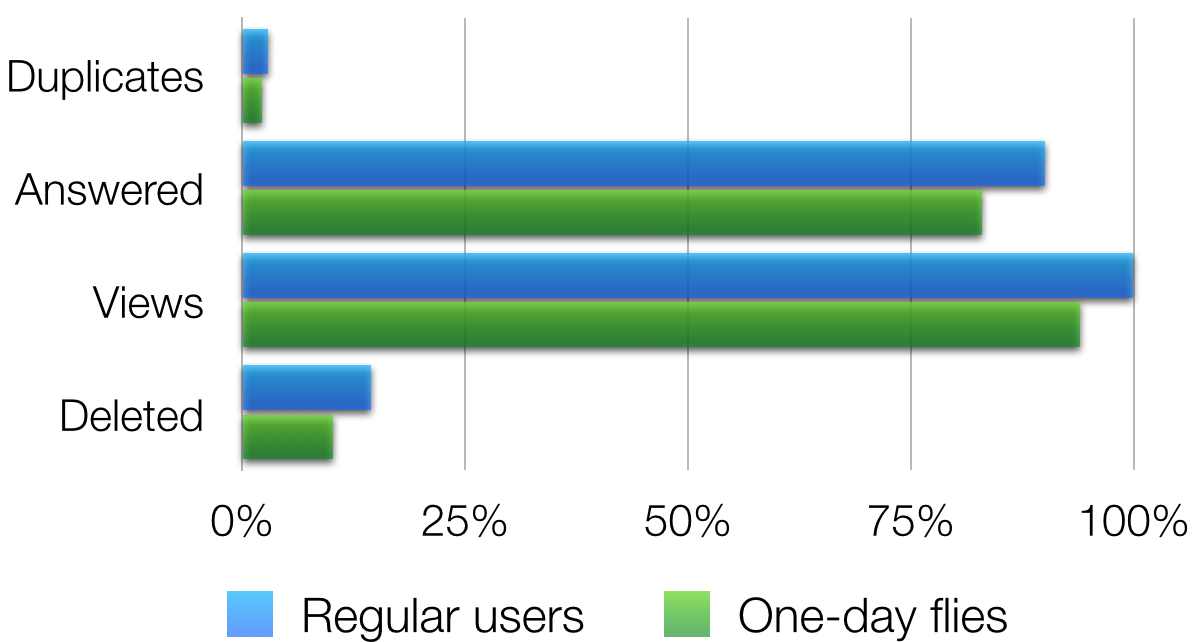
\includegraphics[width=9cm]{BarPlot.png}
 \caption{Results of the analysis}
 \label{finalResults}
\end{figure}

\bibliographystyle{abbrv}
\bibliography{onedayflies}


% that's all folks
\end{document}
